\documentclass[conference]{IEEEtran}
\IEEEoverridecommandlockouts
% The preceding line is only needed to identify funding in the first footnote. If that is unneeded, please comment it out.
\usepackage{cite}
\usepackage{amsmath,amssymb,amsfonts}
\usepackage{algorithmic}
\usepackage{graphicx}
\usepackage{textcomp}
\usepackage{xcolor}
\DeclareMathOperator*{\argmax}{arg\,max}
\def\BibTeX{{\rm B\kern-.05em{\sc i\kern-.025em b}\kern-.08em
    T\kern-.1667em\lower.7ex\hbox{E}\kern-.125emX}}
\begin{document}

\title{A Tensorflow implementation of the Hessian Free Algorithm
%\\
%{\footnotesize \textsuperscript{*}Note: Sub-titles are not captured in Xplore and
%should not be used}
%\thanks{Identify applicable funding agency here. If none, delete this.}
}

\author{\IEEEauthorblockN{Niklas Brunn}
\IEEEauthorblockA{\textit{Albert Ludwigs University of Freiburg} \\
\textit{Mathematical Institute}\\
Freiburg, Germany \\
niklasbrunn@web.de}
\and
\IEEEauthorblockN{No\"{e}l Kury}
\IEEEauthorblockA{\textit{dept. name of organization (of Aff.)} \\
\textit{name of organization (of Aff.)}\\
Freiburg, Germany \\
email address}
\and
\IEEEauthorblockN{Clemens A. Schächter}
\IEEEauthorblockA{\textit{dept. name of organization (of Aff.)} \\
\textit{name of organization (of Aff.)}\\
Freiburg, Germany \\
email address}
}

\maketitle

\begin{abstract}
This report is a written elaboration of a project which was developed in the lecture Numerical Optimization in the winter term 21/22 at the Albert-Ludwigs-University of Freiburg.\\
We discuss a $2^{\text{nd}}$-order optimization method for training deep neural networks using the Generalised Gauss Newton Matrix as an approximation for the Hessian of the objective loss function. This optimization method is superior to $1^{\text{st}}$-order methods, which uses only the gradient of the objective loss function with respect to the Deep Neural Networks`s parameters, in the sense that fewer iterations are required until convergence. Next, we present an implementation of the method using Python, Tensorflow and examine results using a simulated simple dataset and the MNIST dataset.
\end{abstract}

\section{Introduction} 
Deep Neural Networks (DNNs) are one of the main components of Deep Learning which is a subfield of Machine Learning. When training a DNN, the network parameters are updated according to certain rules, which we call the DNN optimization method. By default, the Stochastic Gradient Descent (SGD) method is used as the optimization method. This is a $1^{\text{st}}$-order optimization method in which only the negative gradient of the object loss function (OL) with respect to the network parameters is used to update the current parameters.
One problem of SGD is that pathological curvature is not considered in the OL. This means that the method can get stuck in saddle points, or often converges very slowly in environments with pathological curvature. 
$2^{\text{nd}}$-order optimization methods take into account the curvature of the OL and can thus circumvent such problems, but they are costly in time because second order derivatives must be computed for this purpose. 
We want to use a version of Newton's method for DNN optimization as presented in (MARTENS).
The method presented there uses an approximation of the Hessian matrix, which is positive definite, and thus allows the use of the Conjugate Gradient (CG) method for determining parameter updates. We will therefore go into more detail on the individual problems of standard Newton updates and the improvements proposed for them in order to ensure efficiency.
We also explain how to implement the method in Python with Tensorflow, using the Automatic Differentiation commands provided in the package for forward differentiation and backward differentiation, and provide the reader our own implementation of the method (GITHUBLINK). 


\section{Training Deep Neural Networks as an optimization problem}
In this section, we introduce the necessary mathematical notations for training deep neural networks, formulate the Parameter optimization task as a non-linear-program (NLP) and explain tricks for the Objective Loss Function, which will be useful later when implementing the presented method.\\

\subsection{Deep Neural Networks}
As one of the main components of Deep Learning, DNNs are function approximators that can approximate any continuous function arbitrarily well. Given a dataset of observation pairs $D =\{(x_{i}, y_{i})_{1\leq i\leq N}\}$ with input ${x}$ and corresponding targets $y$, the optimization task is to find optimal parameters such that given an observation $x$, the DNN`s evaluation with current parameters is approximatively the coressponding observed target $y$.  Whenever we use the designation
DNN we actually mean the realisation of a DNN given an input $x$, which is a mapping
$$\mathrm{R}_{x}(\theta):\mathbb{R}^{d}\rightarrow\mathbb{R}^{m},$$
where $\theta$ is a vector containing the parameters of the DNN and $\Theta^{d}=\mathbb{R}^{d}$ denotes the parameter space with usually $d >> m$. We shortly write 
\begin{align} 
\hat{y}_{x} := \mathrm{R}_{x}(\theta)
\end{align}
for the Output of a DNN given an input $x$ with current parameters $\theta$. In detail $\mathrm{R}_{x}$ is an alternating concatenation of a fixed number of affine and non-linear mappings, where the parameter vector $\theta$ is the collection of every entry of all matrices and vectors in the affine mappings. The affine mappings are called Layers and the non-linear mappings are called activation functions in the Machine Learning literature and are always applied element-wise to the output of the preceding Layers. \\
(For a more detailed introduction to DNNs, we provide additional material in the Appendix)\\
Within this report, we also assume that there is no further activation function for DNNs after the last layer but allow that outside the DNN a further activation function $\text{akt}:\mathbb{R}\rightarrow\mathbb{R}$ can be placed after the output, which we will assume to be convex as is the case e.g. in MNIST classification with feed forward DNNs and the softmax-activation function.
In that case we denote the Output of the afterwards (element wise) application of an activationfunction to the output of a DNN with
\begin{align}
z_{x} := \text{akt}(\hat{y}_{x}) = \text{akt}(\mathrm{R}_{x}(\theta)).
\end{align}

\subsection{Loss functions}
For the optimization we need a good optimization criterion in the of a scalar-valued loss function
\begin{align*}
&\mathrm{L}:\mathbb{R}^{m}\rightarrow \mathbb{R}^{+};\\
&(\hat{y}_{x}, y)\mapsto \mathrm{L}_{y}(z_{x}) := \mathrm{L}(z_{x}, y),
\end{align*}
which is assumed to be at least twice continuous-differentiable and convex, for reasons we will discuss later. The loss can be seen as a feedback signal, how well the DNN fits the observation data with its current parameters.

\subsection{Network training formulated as a NLP}
Parameter optimization of a Deep Neural Network can be formulated as an unconstrained NLP. Therefore we define the OL as a mapping which calculates the empirical loss of the DNN`s output with current parameters $\theta$ given the input $x$ and the actual target $y$
\begin{align*}
&f_{D}:\Theta^{d}\rightarrow\mathbb{R}^{+};\\
\theta\mapsto f_{D}(\theta) &:= \mathbb{E}_{D}[\mathrm{L}_{y}(z_{x})] =  \frac{1}{N}\sum_{j = 1}^{N}\mathrm{L}_{y_{j}}(z_{x_{j}}).
\end{align*}
Thus we get the corresponding NLP formulation
$$\argmax_{\theta\in\Theta^{d}}\quad f_{D}(\theta),$$
where $\theta$ denotes the decition variable and $f_{D}$ the objective function of the NLP.
Further, if we consider only one observation $(x, y)$ from the observation data set $D$, then we briefly write  $f_{x, y}$ for the corresponding OL.

\subsection{Matching loss functions}
For later purposes we need to calculate the Jacobian or. the gradient of the OL with respect to the DNN`s parameters. Since the derivative is linear and for simplicity, we consider the OL for only one pair of observations
\begin{align}
\frac{\partial}{\partial\theta}f_{x, y}(\theta) = \mathrm{J}_{f_{x, y}}.
\end{align}
Applying the chain rule we can rewrite it to
\begin{align}
\mathrm{J}_{f_{x, y}} &= \mathrm{J}_{\mathrm{L}_{y}\circ \:\text{akt} \:\circ\:\mathrm{R}_{x}} = \mathrm{J}_{\mathrm{L}_{y}} \: \mathrm{J}_{\text{akt}} \: \mathrm{J}_{\mathrm{R}_{x}},\\
\mathrm{J}_{f_{x, y}}^{\mathrm{T}} &= \mathrm{J}_{\mathrm{R}_{x}}^{\mathrm{T}} \: \mathrm{J}_{\text{akt}}^{\mathrm{T}} \: \mathrm{J}_{\mathrm{L}_{y}}^{\mathrm{T}}.
\end{align}
As (Schraudolph) introduced it in his Article, we also make use of the so-called matching loss functions, where we say that a loss function $\mathrm{L}$ matches the output-non-linearity $\text{akt}$ if
\begin{align}
\frac{\partial}{\partial\hat{y}_{x}}\left(\mathrm{L}_{y}\circ \text{akt}\right)^{\mathrm{T}}(\hat{y}_{x})= \mathrm{J}_{\mathrm{L}_{y}\circ \:\text{akt}}^{\mathrm{T}} = A\: z_{x} + b,
\end{align}
for a matrix $A$ and a vector $b$ which both do not depend on the parameters $\theta$.
The concept of matching loss functions will helpe us later in the implementation of the method. We will also see that many of the well known loss functions used for DNN optimization match their output-non-linearity, e.g. the squared error loss function.


\section{$2^{\text{nd}}$-order optimization}
In this section we want to give the reader a compact presentation of the different components used in the presented method. We will briefly review the Newton`s method and go over the advantages and disadvantages of the Hessian matrix, and then introduce the necessary theory for the efficient $2^{\text{nd}}$-order optimization method.

\subsection{Newton's method}\label{AA}
As mentioned before, Newton`s method is an optimization method, where we update the decition variables of a NLP iteratively by
\begin{align}
 \theta_{k+1} = \theta_{k} + t\cdot (-\mathrm{H}_{f_{x, y}}^{-1}\:\mathrm{J}_{f_{x, y}}^{\mathrm{T}}),
\end{align}
where $\mathrm{H}_{f_{x, y}}$ denotes the always symmetric hessian matrix of the OL with respect to the current DNN`s parameters $\theta$ in the $k+1$-th step and for some scalar value $t$, representing the learning rate. In practice we set the learning rate constant to $t=1$. This approach is motivated by minimize the local quadratic approximation
\begin{align}
q(\theta + \delta)_{x, y} := f_{x, y}(\theta) + \mathrm{J}_{f_{x, y}}^{\mathrm{T}}\:\delta + \frac{1}{2}\:\delta^{\mathrm{T}}\:\mathrm{H_{f_{x, y}}}\:\delta \approx f_{x, y}(\theta + \delta).
\end{align}
with respect to $\delta$. 
Respecting informations about the curvature of the OL, using the hessian can in contrast to the usage of gradient descent lead to convergence in much lesser iterations because it rescales the gradient of the OL in every step.

\subsection{Problems with the Hessian}
We implicitly assume in every step of the Newton`s methode that the Hessian matrix is invertible, which in our case is very rare in the task of optimizing DNN`s parameters and even if the Hessian is invertible, we cannot ensure converges to a local minimum, since the Hessian usually does not have to be positive semidefinite either. Apart from that, the Hessian matrix has $d^{2}$ entries when optimizing DNNs, which makes it incredibly expensive to calculate, assuming $d>>m$. For this reason, the direct application of Newton's method to our task is inappropriate and we must first make some modifications.

\subsection{The Generalized Gauss Newton Matrix}
As a first improvement, we no longer use the Hessian matrix itself, but the Generalized Gauss Newton matrix (GGN), which is an approximation of the Hessian matrix
\begin{align}
\mathrm{G}_{f_{x, y}} := \mathrm{J}_{\hat{y}_{x}}^{\mathrm{T}}\:\mathrm{H}_{\mathrm{L_{y}\circ\:\text{akt}}}\:\mathrm{J}_{\hat{y}_{x}},
\end{align}
with $\mathrm{H}_{\mathrm{L_{y}\circ\:\text{akt}}}$ denoting the hessian of $\mathrm{L_{y}\circ\:\text{akt}}$ with respect to the DNN`s output $\hat{y}_{x}$.
This representation is motivated by the fact that in the representation of the complete Hessian matrix
\begin{align}
\mathrm{J}_{\hat{y}_{x}}^{\mathrm{T}}\:\mathrm{H}_{\mathrm{L_{y}\circ\:\text{akt}}}\:\mathrm{J}_{\hat{y}_{x}}\:\sum_{j = 1}^{m}\left(\left(\mathrm{J}_{\mathrm{L}_{y}\circ \:\text{akt}}^{\mathrm{T}}\right)_{j}\cdot\mathrm{H}_{(\hat{y}_{x})_{j}}\right),
\end{align}
where $\mathrm{H}_{(\hat{y}_{x})_{j}}$ denotes the hessian of the DNN`s  $j$-th output, the last sum-term vanishes if 
$$\left(\mathrm{J}_{\mathrm{L}_{y}\circ \:\text{akt}}^{\mathrm{T}}\right)_{j}\approx 0,$$
which means that in this case the network represents the targets well.  Moreover, the GGN is a symmetric matrix and is positive semidefinite for non-decreasing convex loss functions since for every $v\in\mathbb{R}^{d}$ and from the convexity of $\mathrm{L_{y}\circ\:\text{akt}}$ it holds that
\begin{align}
v^{\mathrm{T}}\:\mathrm{G}_{f_{x, y}}\:v &= v^{\mathrm{T}}\:\left( \mathrm{J}_{\hat{y}_{x}}^{\mathrm{T}}\:\mathrm{H}_{\mathrm{L_{y}\circ\:\text{akt}}}\:\mathrm{J}_{\hat{y}_{x}}\right)\:v\\
&= \left(\mathrm{J}_{\hat{y}_{x}\:v}\right)^{\mathrm{T}}\:\mathrm{H}_{\mathrm{L_{y}\circ\:\text{akt}}}\left(\mathrm{J}_{\hat{y}_{x}\:v}\right) \\
&\geq 0.
\end{align}
Note that in the case, where the extra activation function is not convex, we can also place the aktivation function behind the last Layer of the DNN resulting in a more general formulation of the GGN
\begin{align}
\mathrm{G}_{f_{x, y}} = \mathrm{J}_{\hat{y}_{x}}^{\mathrm{T}}\:\mathrm{H}_{\mathrm{L_{y}}}\:\mathrm{J}_{\hat{y}_{x}},
\end{align}
where the above discussed properties remain due to the convexity of the loss function.
This 
\subsection{Levenberg-Marquardt algorithm }
Even if we replace the hessian with the symmertic and positive semidefinite GNN in the steps of the above presented Newton`s method, it is sometimes the case that this matrix is also not invertible and therefore we cant compute a solution of the non-linear system 
\begin{align}
\mathrm{H}_{f_{x, y}}\cdot(\theta_{k+1} - \theta_{k}) = -t\cdot\mathrm{J}_{f_{x, y}}^{\mathrm{T}},
\end{align}
which is equivalent to finding a solution of the system [entsprechende Nummer von Oben; Abschnit Newton`s Method].
For that reason we use a damped version of the GGN (DGGN) where we add an additional positive definite diagonal matrix with sufficient large enough values on the diagonal, e.g.
\begin{align}
\mathrm{DG}_{f_{x, y}} := \mathrm{G}_{f_{x, y}} + \lambda\cdot\mathrm{I}^{d\times d},
\end{align}
with $\mathrm{I}^{d\times d}$ denoting the $d\times d$ unit matrix and some $\lambda>0$.
The DGGN constructed in this way is then actually invertible. 
To see this we consider the decomposition
\begin{align}
\mathrm{G}_{f_{x, y}} = \mathrm{U}\:\Lambda\:\mathrm{U}^{\mathrm{T}},
\end{align}
with an orthogonal Matrix $\mathrm{U}\in\mathbb{R}^{d\times d}$ and a diagonal Matrix $\Lambda\in\mathbb{R}^{d\times d}$ which on the diagonal entries contains the non-negative eigenvalues of the GGN. This decomposition exists because the GGN is symmetric and positive semidefinite. Further it holds that
\begin{align}
\mathrm{DG}_{f_{x, y}} &= \mathrm{U}\:\Lambda\:\mathrm{U}^{\mathrm{T}} + \lambda\cdot\mathrm{I}^{d\times d}\\
&= \mathrm{U}\:\Lambda\:\mathrm{U}^{\mathrm{T}} + \mathrm{U}\:\lambda\cdot\mathrm{I}^{d\times d}\:\mathrm{U}^{\mathrm{T}}\\
&= \mathrm{U}\:\left(\Lambda + \lambda\cdot\mathrm{I}\right)\:\mathrm{U}^{\mathrm{T}}
\end{align}
where the Matrix $\left(\Lambda + \lambda\cdot\mathrm{I}\right)$ is a diagonal one with only positive entries on the diagonal. Therefore the determinant of the produkt of the matrices in the last term is positive and as a consequence we get that the DGGN is invertible.
Note that a choice of $\lambda>>0$ leads to a Newton step where we would nearly not move away from our current parameters if $t = 1$, while a choice of $\lambda\approx 0$ leads to a full step using the GGN [als Quelle zum Nachlesen hier vllt. das Vorlesungsskript angeben, Kapitel 6.7]. In practice, we update the value $\lambda$ after each iteration step according to certain conditions which we will explain in more detail later.
\\TODO ... (warum ist die resultierende Matrix dann invertierbar noch hinzufügen ...)
\subsection{Conjugate gradient method}
TODO ... (CG Erklären, R-Op. und effiziente Matrix-V-P., CG-Methode Extras erklären)

\section {Implementation}

\subsection{Authors and Affiliations}
\textbf{The class file is designed for, but not limited to, six authors.} A 
minimum of one author is required for all conference articles. Author names 
should be listed starting from left to right and then moving down to the 
next line. This is the author sequence that will be used in future citations 
and by indexing services. Names should not be listed in columns nor group by 
affiliation. Please keep your affiliations as succinct as possible (for 
example, do not differentiate among departments of the same organization).

\subsection{Identify the Headings}
Headings, or heads, are organizational devices that guide the reader through 
your paper. There are two types: component heads and text heads.

Component heads identify the different components of your paper and are not 
topically subordinate to each other. Examples include Acknowledgments and 
References and, for these, the correct style to use is ``Heading 5''. Use 
``figure caption'' for your Figure captions, and ``table head'' for your 
table title. Run-in heads, such as ``Abstract'', will require you to apply a 
style (in this case, italic) in addition to the style provided by the drop 
down menu to differentiate the head from the text.

Text heads organize the topics on a relational, hierarchical basis. For 
example, the paper title is the primary text head because all subsequent 
material relates and elaborates on this one topic. If there are two or more 
sub-topics, the next level head (uppercase Roman numerals) should be used 
and, conversely, if there are not at least two sub-topics, then no subheads 
should be introduced.

\subsection{Figures and Tables}
\paragraph{Positioning Figures and Tables} Place figures and tables at the top and 
bottom of columns. Avoid placing them in the middle of columns. Large 
figures and tables may span across both columns. Figure captions should be 
below the figures; table heads should appear above the tables. Insert 
figures and tables after they are cited in the text. Use the abbreviation 
``Fig.~\ref{fig}'', even at the beginning of a sentence.

\begin{table}[htbp]
\caption{Table Type Styles}
\begin{center}
\begin{tabular}{|c|c|c|c|}
\hline
\textbf{Table}&\multicolumn{3}{|c|}{\textbf{Table Column Head}} \\
\cline{2-4} 
\textbf{Head} & \textbf{\textit{Table column subhead}}& \textbf{\textit{Subhead}}& \textbf{\textit{Subhead}} \\
\hline
copy& More table copy$^{\mathrm{a}}$& &  \\
\hline
\multicolumn{4}{l}{$^{\mathrm{a}}$Sample of a Table footnote.}
\end{tabular}
\label{tab1}
\end{center}
\end{table}

\begin{figure}[htbp]
\centerline{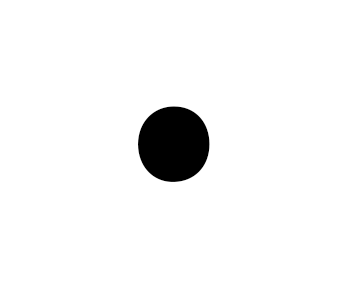
\includegraphics{fig1.png}}
\caption{Example of a figure caption.}
\label{fig}
\end{figure}

Figure Labels: Use 8 point Times New Roman for Figure labels. Use words 
rather than symbols or abbreviations when writing Figure axis labels to 
avoid confusing the reader. As an example, write the quantity 
``Magnetization'', or ``Magnetization, M'', not just ``M''. If including 
units in the label, present them within parentheses. Do not label axes only 
with units. In the example, write ``Magnetization (A/m)'' or ``Magnetization 
\{A[m(1)]\}'', not just ``A/m''. Do not label axes with a ratio of 
quantities and units. For example, write ``Temperature (K)'', not 
``Temperature/K''.

\section{Experiments}

\subsection{Simple simulated data}
...

\subsection{MNIST}
...

\section*{Acknowledgment}

The preferred spelling of the word ``acknowledgment'' in America is without 
an ``e'' after the ``g''. Avoid the stilted expression ``one of us (R. B. 
G.) thanks $\ldots$''. Instead, try ``R. B. G. thanks$\ldots$''. Put sponsor 
acknowledgments in the unnumbered footnote on the first page.


\begin{thebibliography}{00}
\bibitem{b1} Moritz Diehl, "Lecture Notes on Numerical Optimization (Preliminary Draft)", Albert Ludwigs University of Freiburg, September 29, 2017	
\bibitem{b2} James Martens, "Deep learning via Hessian-free optimization", University of Toronto, Ontario, M5S 1A1, Canada, 2010
\bibitem{b3} James Martens, "New Insights and Perspectives on the Natural Gradient Method", Jurnal of Machine Learning Research 21, arXiv:1412.1193v11 [cs.LG], September 19, 2020
\bibitem{b4} Nicol N. Schraudolph, "Fast Curvature Matrix-Vector Products for Second-Order
Gradient Descent", Neural Computation, August 2002
\end{thebibliography}

\end{document}
